\section{Komplexe Zahlen}
\subsection{Operationen}
\subsubsection{Kartesisch}
In diesem Koordinatensystem lassen sich \textit{Addition} und \textit{Subtraktion} besonders einfach lösen!

\noindent\textbf{Addition}\\
$(a_1 + ja_2) + (b_1 + jb_2) = a_1 + ja_2 + b_1 + jb_2 = (a_1 + b_1) + j(a_2 + b_2)$\\
\noindent\textbf{Subtraktion}\\
$(a_1 + ja_2) - (b_1 + jb_2) = a_1 + ja_2 - b_1 - jb_2 = (a_1 - b_1) + j(a_2 - b_2)$\\
\noindent\textbf{Multiplikation} (Binom.)\\
$(a_1 + ja_2) \cdot (b_1 + jb_2) = (a_1b_1 - a_2b_2) + j(a_1b_2 + a_2b_1)$\\
\noindent\textbf{Division}\\
$\frac{a_1 + ja_2}{b_1 + jb_2} = \frac{(a_1 + ja_2)(b_1 - jb_2)}{(b_1 + jb_2)\underbrace{(b_1 - jb_2)}_{\text{Ergänzung}}} = \frac{1}{b_1^2 + b_2^2}(a_1+ja_2)(b_1 - jb_2)$\\
\noindent\textbf{Potenz}\\
$e^a\cdot e^b = e^{a+b}; \frac{e^a}{e^b} = e^{a-b}; (e^a)^b = e^{a\cdot b}; $

\todo{Hinweis: Bei komplizierten Winkeln ggf. auch eine Gleichungssystem aufstellen.}

\subsubsection{Polar}
In diesem Koordinatensystem lassen sich \textit{Multiplikation} und \textit{Division} besonders einfach lösen!

\noindent\textbf{Multiplikation}\\
$\Re(z) = a_1 \cdot b_1; \Im(z) = \arg(a_2 \cdot b_2) = \arg(a_2) + \arg(b_2)$\\

\noindent\textbf{Division}\\
$\Re(z) = \frac{a_1}{b_1}; \Im(z) = \arg(\frac{a_2}{b_2}) = \arg(a_2) - \arg(b_2)$\\



\includegraphics[width=0.7\linewidth]{Images/screenshot004}

\includegraphics[width=0.7\linewidth]{Images/screenshot005}
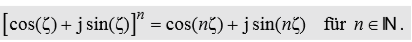
\includegraphics[width=0.7\linewidth]{Images/screenshot003}
\todo{Pro n-te Wurzel eine Lösung!}
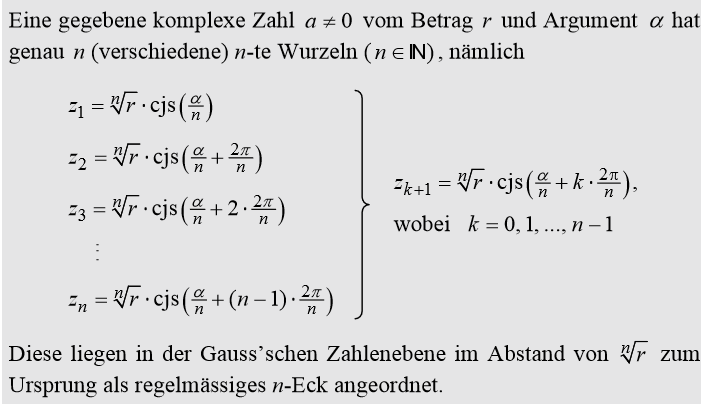
\includegraphics[width=0.7\linewidth]{Images/screenshot006}


\subsection{Polarform Umwandlung}
\todo{ACHTUNG: Re(z) < 0!!}
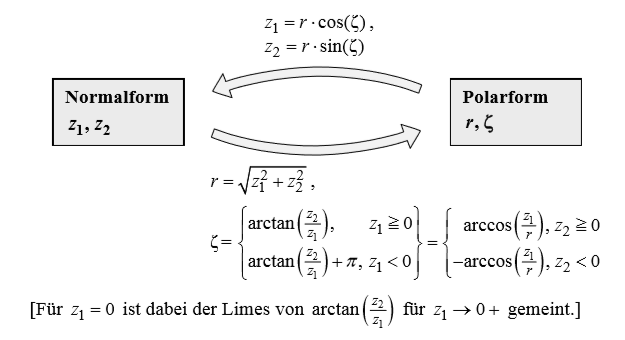
\includegraphics[width=0.7\linewidth]{Images/screenshot002}

\subsubsection{Trigo}
\todo{Einheitskreis mit Tangens und Gleichseitige/Schenklige Dreiecke (Wurzel 2 etc)}
Punkte auf Kreis ($\cos\phi$, $\sin\phi$)\\
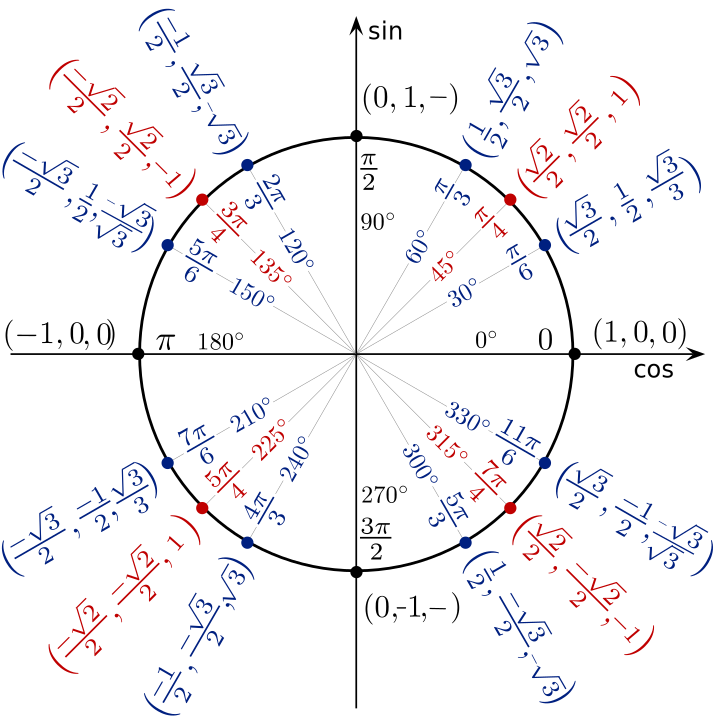
\includegraphics[width=0.7\linewidth]{Images/einheitskreis}
